\chapter{Visualization Methods}
\label{Chapter2}

We take up ordinary perspective cameras for surveillance cameras in this research.

%------------------------------------------------------------------------------

\section{Visualization Elements}
\label{VisualizationRequirements}

Viewing volume of a projective camera is defined by an infinite half cone, apex of which corresponds to the focal point of the camera. Because real computers cannot have unlimited resources, in practical computer 3D technology we usually limit the bottom of the cone by a far clip plane or by a boundary surface which may cut the viewing volume, then limit the top of the cone even more by a near clip plane. It may result in a frustum (figure \ref{fig:ViewingVolume}). Thus in this research we abstract the viewing volume for visualization by the term ``viewing field''.

\begin{figure}[htbp]
	\centering
	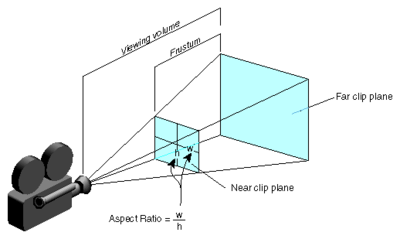
\includegraphics{./Primitives/viewing_volume.png}
	\rule{35em}{0.5pt}
	\caption[Viewing volume of camera]{Viewing volume of camera}
	\label{fig:ViewingVolume}
\end{figure}

There may be many methods for visualizing the viewing fields, not limited to the ones discussed in the next section. But for a method to find practical use in outdoor MR, it should be able to be implemented (see section \ref{UseCases} to have a rough illustration) so that it meets the following basic qualitative requirements, expressed in the ``it should'' tongue of most Domain Specific Language of the Behavior Driven Development methodology in software engineering:

\begin{itemize}
	\item It should be easy to understand when users see the visualized viewing fields of surrounding surveillance cameras.
	\item It should work in realtime. When the user changes the position or orientation of the mobile device, the MR video displayed on the screen of the mobile device should simultaneously change accordingly to the movement with no or little delay.
	\item It should have good accuracy. In order to correctly overlay CG objects onto the original video taken at the user side, the position and orientation of the mobile camera must be estimated within a small error.
	\item It should be robust to disturbance in outdoor environment. Some of the disturbance that may arise in real situations are passers in front of the camera and GPS signal noise/weakness. For example, in outdoor environment, there may be bicycle riders passing by and they may temporary occlude the camera. Another example is that if the system use GPS device, the GPS signal strength may change a lot when the user walk from an open space to a space shadowed by trees or buildings.
\end{itemize}

We must take the above requirements into account when implementing the prototype in chapter \ref{Chapter3} and conducting experiment to evaluate the visualization methods.

%------------------------------------------------------------------------------

\section{Visualization Methods}
\label{VisualizationMethods}

This section discusses the idea of five visualization methods. Chapter \ref{Chapter3} will implement and integrate them into a working prototype. Chapter \ref{Chapter4} will conduct an experiment to evaluate them.

\subsection{Volume Method}

As discussed above, the natural method to visualize the viewing field is simply visualizing the viewing volume (figure \ref{fig:VolumeMethod}). However, the volume usually occludes parts of the mobile device's screen, especially if the user is inside the viewing volume, hence may be hard to understand.

\begin{figure}[htbp]
	\centering
	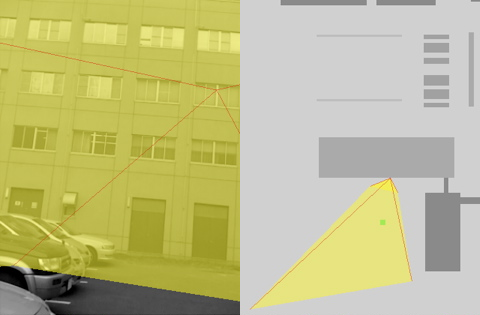
\includegraphics{./Primitives/theory_volume.png}
	\rule{35em}{0.5pt}
	\caption[Volume method]{Volume method}
	\label{fig:VolumeMethod}
\end{figure}

\subsection{Shadow Method}

The fact that the frame captured by the camera is perspective projection of the volume into the near plane of the frustum gives us another method. This method visualizes the virtual shadow created by the light positioned at the eye-point of the camera and the near plane of the frustum (figure \ref{fig:ShadowMethod}). This method may give more understandable visualization. There are various ways to render the shadow, the two popular ones are shadow mapping \cite{Reference7} \cite{Reference8} and volume shadow \cite{Reference9}.

\begin{figure}[htbp]
	\centering
	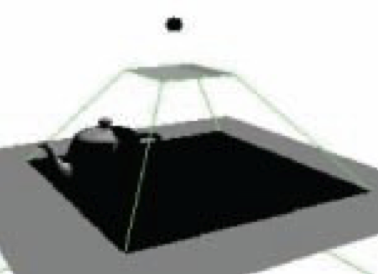
\includegraphics{./Primitives/theory_shadow.png}
	\rule{35em}{0.5pt}
	\caption[Shadow method]{Shadow method}
	\label{fig:ShadowMethod}
\end{figure}

\subsection{Contour Method}

An alternative method is to only visualize the contours of the shadow (figure \ref{fig:ContourMethod}) to reduce the occlusion of the CG object. Rendering only the contour is much lighter than rendering the whole shadow, thus this method is supposed to be much faster.

\begin{figure}[htbp]
	\centering
	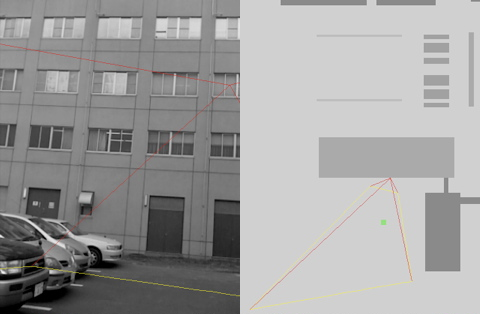
\includegraphics{./Primitives/theory_contour.png}
	\rule{35em}{0.5pt}
	\caption[Contour method]{Contour method}
	\label{fig:ContourMethod}
\end{figure}

\subsection{Vector Method}

For most of the time, a person may want to know not only the viewing field, but also the position and distance to the surveillance camera, To visualize this information, we propose a method using vectors (figure \ref{fig:VectorMethod}). In the figure, all the vectors are pointing the camera, and the length of the vectors are reverse proportional to the distance from the root of the vectors to the camera.

\begin{figure}[htbp]
	\centering
	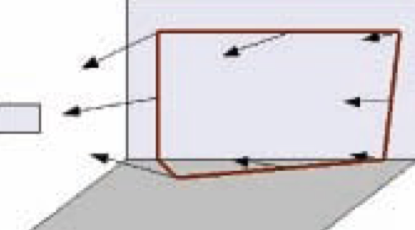
\includegraphics{./Primitives/theory_vector.png}
	\rule{35em}{0.5pt}
	\caption[Vector method]{Vector method}
	\label{fig:VectorMethod}
\end{figure}

\subsection{Animation Method}

This method uses moving CG objects (figure \ref{fig:AnimationMethod}) coming from the surveillance cameras to the ground (or vice versa from the ground to the cameras) to to visualize the viewing fields. This method has  many advantages:

\begin{itemize}
	\item The moving CG objects start from the surveillance camera positions (or move towards the cameras). As a result the user easily knows the camera positions.
	\item Even when the mobile device is fixed at a certain position and orientation, the visualization effect is still achieved because of the moving CG objects.
	\item The moving CG objects do not occlude the scene. As a result the user can easily see the scene and the visualized camera viewing fields at the same time.
\end{itemize}

\begin{figure}[htbp]
	\centering
	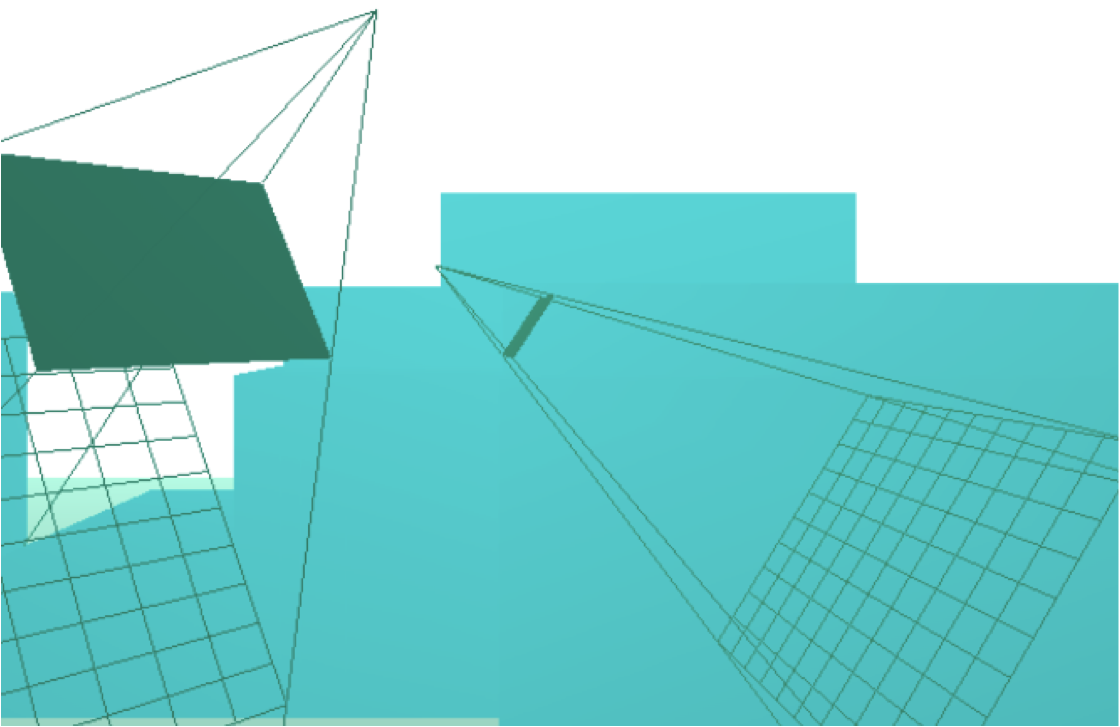
\includegraphics[width=10cm]{./Primitives/theory_animation.png}
	\rule{35em}{0.5pt}
	\caption[Animation method]{Animation method}
	\label{fig:AnimationMethod}
\end{figure}
